\chapter{Tests des Robotersystems}
\label{cha:Tests}

\section{Realtests}

Das kontrollierte Testen eines Roboters ist nicht ganz leicht. Aufgrund der Abhängigkeiten zwischen Hard- und Software reichen reine Software-basierte Tests hier nicht aus. Bei der Übertragung der Befehle für Bewegung des Roboters beispielsweise muss auch tatsächlich der Roboter vorhanden und betriebsbereit sein, die Befehle müssen über eine bestehende Bluetooth-Verbindung an ihn übertragen und schließlich dessen Reaktion beobachtet werden.

Deshalb wurde häufig auf die Methode des Ausprobierens (\enquote{Trial and Error}) zurückgegriffen. Sobald eine Komponente wie die Objekterkennung als ganzes geschrieben war und kompilierte, wurde die App auf das Smartphone geladen und an echten Objekten getestet.

Angefangen hat dies mit einfachen Versuchen in OpenCV, wie eine simple Erkennung der Farbe der Objekte vor der Linse. Hat dies nicht funktioniert, wurden die Parameter angepasst, also beispielsweise die Schwelle der Farbstärke des Erkennungsalgorithmus erhöht und danach erneut ausgeführt. 

Auf diese Art wurde nach und nach um Objektverfolgung durch Kategorisierung und Erkennung der Form erweitert und die gut funktionierende Objekterkennung entwickelt wie sie nun in Betrieb ist.

Ebenso verhielt es sich mit der Ansteuerung der Motoren. Zunächst wurde der Grundaufbau des Roboters zum Testen mit einer im Play-Store erhältlichen allgemeinen Fernsteuerungs-App für NXT-Roboter \enquote{NXT Remote Control} \cite{nxt_remote_control} verwendet. Sie bietet nach Verbindungsaufnahme Bedienelemente zum ansteuern jedes Motors an, was erste Fahrversuche des CLEEN-R-Roboters erlaubte. So wurde auch festgestellt, das der bestehende Aufbau die gestellten Anforderungen in Hinsicht auf Bewegungsfreiheit und Fähigkeit zur Objektaufnahme erfüllt und das Fahrgestell oder der Greifarm nicht weiter verändert werden muss.

Funktionierten mal Motoren oder die Bluetooth-Kommunikation nicht mehr, konnte mit NXT Remote Control auch ständig geprüft werden, ob der Fehler in der Hardware (Stromversorgung unzureichend, Bluetooth am NXT-Modul deaktiviert) oder in der Software (falsche Geschwindigkeit, abgebrochene Verbindung) lag und dementsprechend behoben werden.

Schließlich konnte so durch Ausprobieren, Optimieren und Erweitern unabhängig voneinander Steuerung und Objekterkennung nach und nach erarbeitet, letztendlich zusammengefügt und mit dem Roboter-Aufbau getestet werden.

\section{Manuelle Steuerung}

Zum Testen der Fahrfähigkeit, des Greifarms und hauptsächlich der Positionsverfolgung wurde unter dem Einstellungsmenü der CLEEN-R App der Menüpunkt \enquote{manual control} hinzugefügt. Über ihn wird die in Bild \ref{fig:manualControl} gezeigte Activity gestartet, die dem Benutzer oder Tester die Kontrolle über die Bewegungen des Roboters gibt.

\begin{figure}[h]
\centering
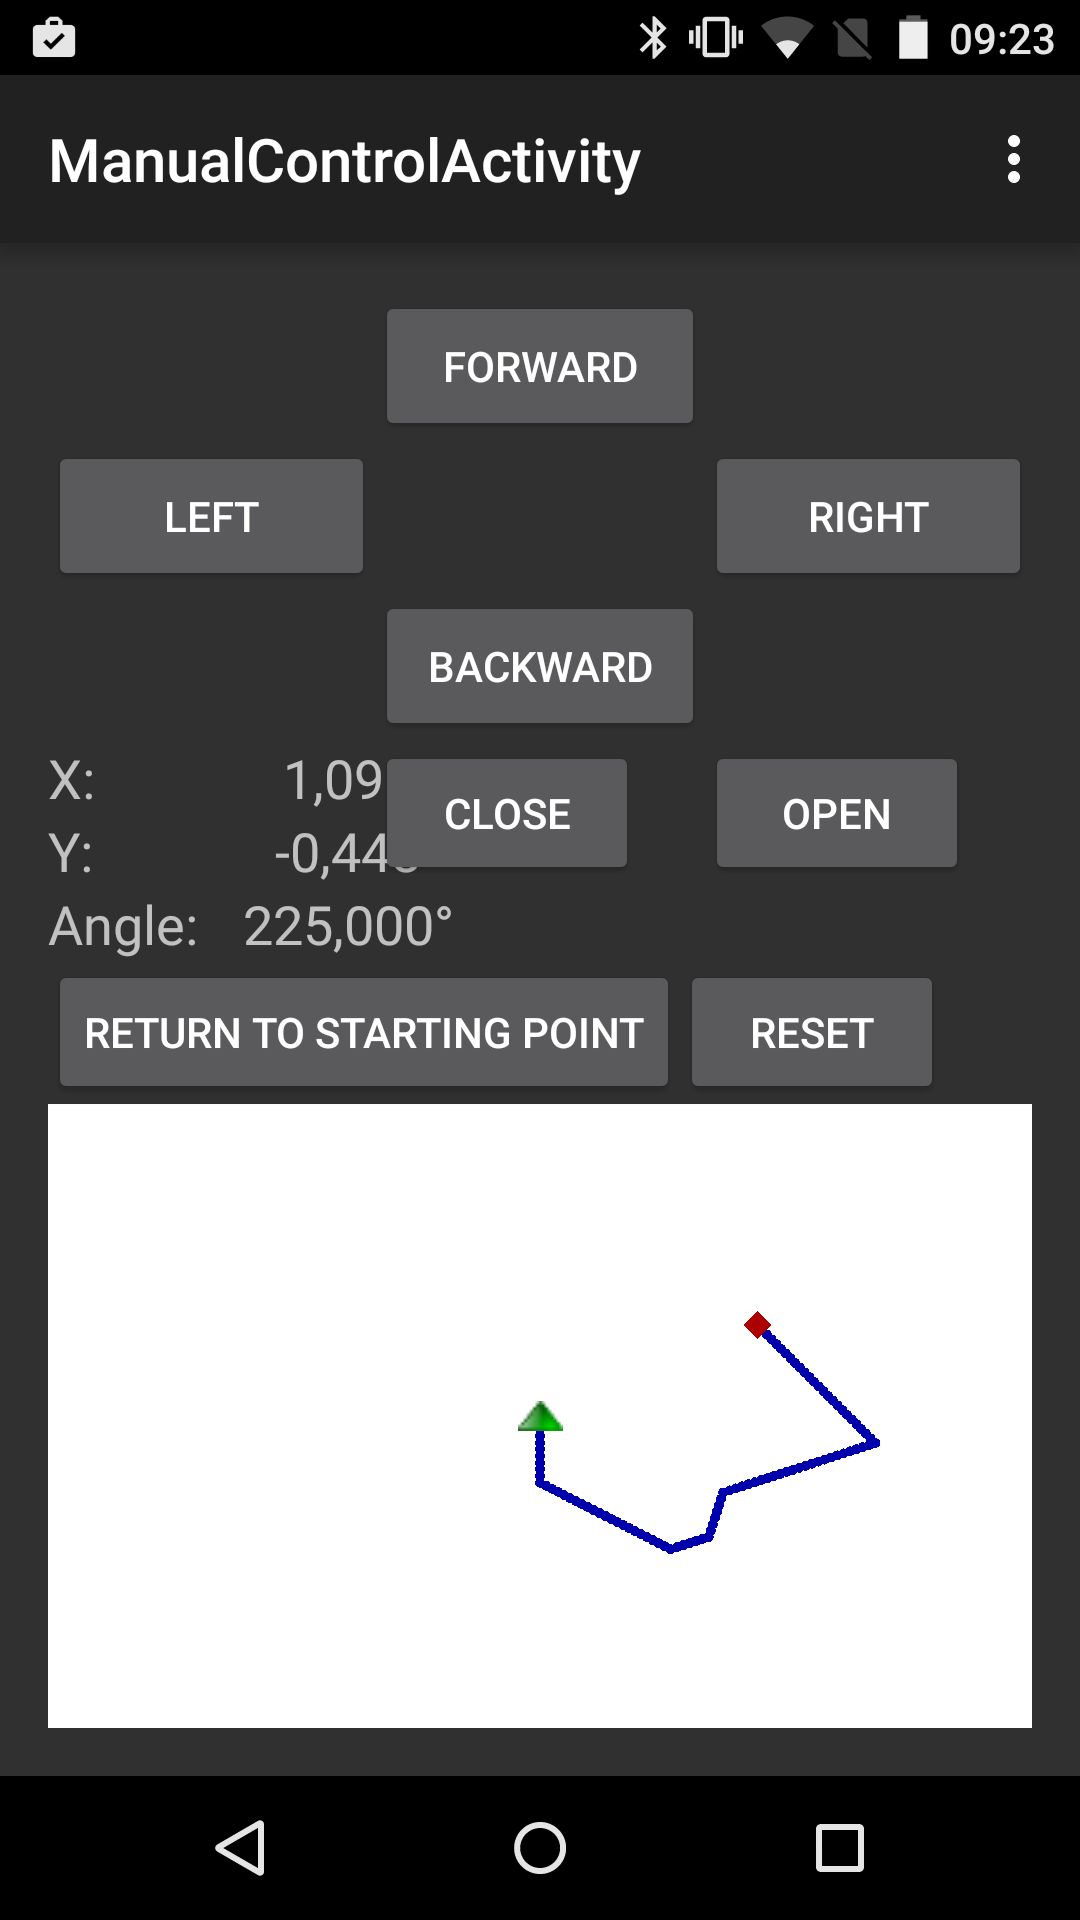
\includegraphics[width=0.4\textwidth]{Bilder/Tests/manualControl}
\caption{Manuelle Steuerung des Roboters}
\label{fig:manualControl}
\end{figure}

Das Smartphone wird für die direkte Kontrolle vom Roboter in die Hand genommen, die Übertragung der Befehle erfolgt wie im Normalbetrieb via Bluetooth.

Über Buttons kann sowohl vor- und rückwärts gefahren, als auch im und gegen den Uhrzeigersinn rotiert werden. Des Weiteren lässt sich der Greifarm beliebig weit öffnen und schließen. Die aktuelle Position und der Winkel im Vergleich zum Start wird in Koordinatenform angezeigt und während der Bewegungen aktualisiert.

Im unteren Teil des Bildschirms befindet sich eine graphische Repräsentation des Roboters und des bereits zurückgelegten Weges durch das Zimmer, der Startpunkt wird ebenfalls markiert.

Nach dem manuellen Anfahren und Aufnehmen eines Objekts kann über den Knopf \enquote{Return to starting point} der Roboter wie in Kapitel \ref{sec:Rückkehr} vollautomatisch zum Startpunkt zurückgefahren werden. Über \enquote{Reset} wird die aktuelle Position des NXT-Roboters zurückgesetzt und als neuer Startpunkt festgelegt.
